    \begin{align}
	    \vec{m} = \myvec{1\\ \tan 75\degree}
	    \implies \vec{n} &= \myvec{2+\sqrt{3}\\-1}
        \label{eq:11/10/2/4normal-vec}
	\\
	    \implies \myvec{2+\sqrt{3} & -1}\vec{x} &=\myvec{2+\sqrt{3}& -1}\myvec{2\\2\sqrt{3}}  
	    \\
	    &= 4
        \label{eq:11/10/2/4line}
    \end{align}
is the desired equation. 
\iffalse
See \figref{fig:11/10/2/4line}.
    \begin{figure}[H]
        \centering
        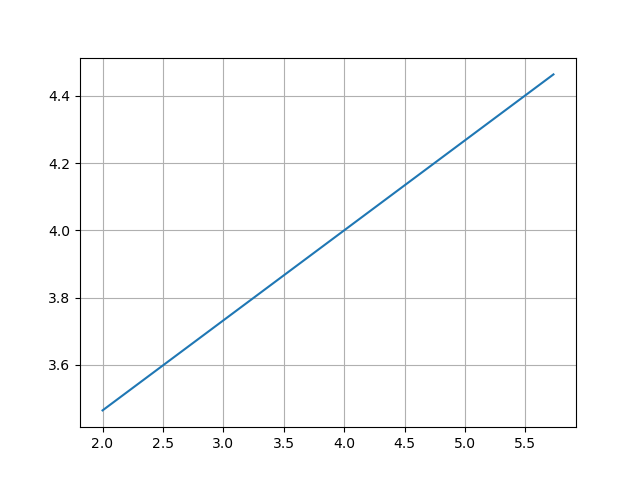
\includegraphics[width=0.75\columnwidth]{chapters/11/10/2/4/figs/line.png}
        \caption{}
        \label{fig:11/10/2/4line}
    \end{figure}
    \fi
